%%%%%%%%%%%%%%%%%%%%%%%%%%%%%%% COMMENT THIS TO COMPILE main.tex %%%%%%%%%%%%%%%%%%%%%%%%%%%%%%%%
\documentclass[a4paper,12pt]{report}
\usepackage[english]{babel}
\usepackage[left=2cm,right=2cm,top=2cm,bottom=2cm]{geometry}
%\usepackage{mathtools}
\usepackage{amsthm}     % for definitions and theorems
\usepackage[many]{tcolorbox}    % boxes around definitions and theorems
%\usepackage{amsmath}
%\usepackage{nccmath}
\usepackage{amssymb}    % \ltimes
\usepackage{etoolbox}   % for start of Chapter
%\usepackage{amsfonts}
\usepackage{physics}    % for all Physics related
\usepackage{dsfont}     % for the identity matrix symbol \1
%\usepackage{mathrsfs}

\usepackage{titling}
\usepackage{indentfirst}

\usepackage{bm}
\usepackage[dvipsnames]{xcolor}
\usepackage{cancel}

\usepackage{xurl}
\usepackage[colorlinks=true]{hyperref}

\usepackage{float}
\usepackage{graphicx}
\usepackage{subcaption}
%\usepackage{tikz}

\usepackage{ctable}     % tabelas
\renewcommand{\P}{\phantom{+}}  % empty space to indent things
\usepackage{multirow}
\usepackage{tabulary}

%%%%%%%%%%%%%%%%%%%%%%%%%%%%%%%%%%%%%%%%%%%%%%%%%%%

\newcommand{\eps}{\epsilon}
\newcommand{\vphi}{\varphi}
\newcommand{\cte}{\text{cte}}

\newcommand{\N}{{\mathbb{N}}}
\newcommand{\Z}{{\mathbb{Z}}}
%\newcommand{\Q}{{\mathbb{Q}}}
\newcommand{\C}{{\mathbb{C}}}
\renewcommand{\S}{{\hat{S}}}
%\renewcommand{\H}{\s{H}}

\renewcommand{\a}{{\vb{a}}}
\renewcommand{\b}{{\vb{b}}}
\renewcommand{\d}{{\dagger}}
\newcommand{\up}{{\uparrow}}
\newcommand{\down}{{\downarrow}}
\newcommand{\hc}{{\text{h.c.}}}

\newcommand{\ihat}{\bm{\hat{\imath}}}
\newcommand{\jhat}{\bm{\hat{\jmath}}}
\newcommand{\khat}{\bm{\hat{k}}}

\newcommand{\0}{{\vb{0}}}
\newcommand{\1}{\mathds{1}}
\newcommand{\E}{{\vb{E}}}
\newcommand{\B}{{\vb{B}}}
\renewcommand{\u}{{\vb{u}}}
\renewcommand{\v}{{\vb{v}}}
\renewcommand{\r}{{\vb{r}}}
\newcommand{\R}{{\vb{R}}}
\newcommand{\Q}{{\vb{Q}}}
\newcommand{\G}{{\vb{G}}}
\newcommand{\g}{{\vb{g}}}
\renewcommand{\k}{{\vb{k}}}
\newcommand{\K}{{\vb{K}}}
\newcommand{\p}{{\vb{p}}}
\newcommand{\q}{{\vb{q}}}
\newcommand{\F}{{\vb{F}}}
\renewcommand{\t}{{\vb{t}}}
\newcommand{\vtau}{{\bm{\tau}}}
\newcommand{\vdelta}{{\bm{\delta}}}

% COLORED SYMMETRY ELEMENTS
\newcommand{\Ct}{{\textcolor{Cyan}{C_3}}}
\newcommand{\Ctn}[1]{{\textcolor{Cyan}{C_3^{\textcolor{black}{#1}}}}}
\newcommand{\Cs}{{\textcolor{ForestGreen}{C_6}}}
\newcommand{\Csn}[1]{{\textcolor{ForestGreen}{C_6^{\textcolor{black}{#1}}}}}
\newcommand{\sd}{{\textcolor{RoyalBlue}{\sigma_d}}}
\newcommand{\sdn}[1]{{\textcolor{RoyalBlue}{\sigma_d^{\textcolor{black}{#1}}}}}
\newcommand{\sdp}{{\textcolor{RoyalBlue}{\sigma_d'}}}
\newcommand{\sdpp}{{\textcolor{RoyalBlue}{\sigma_d''}}}
\newcommand{\sv}{{\textcolor{Orange}{\sigma_v}}}
\newcommand{\svn}[1]{{\textcolor{Orange}{\sigma_v^{\textcolor{black}{#1}}}}}
\newcommand{\svp}{{\textcolor{Orange}{\sigma_v'}}}
\newcommand{\svpp}{{\textcolor{Orange}{\sigma_v''}}}

\newcommand{\s}{\sigma}
%\newcommand{\prodint}[2]{\left\langle #1 , #2 \right\rangle}
\newcommand{\cc}[1]{\overline{#1}}
\newcommand{\Eval}[3]{\eval{\left( #1 \right)}_{#2}^{#3}}
\newcommand{\sg}[2]{\{ #1 \mid #2 \}}

\newcommand{\unit}[1]{\; \mathrm{#1}}

\newcommand{\n}{\medskip}
\newcommand{\e}{\quad \mathrm{and} \quad}
\newcommand{\ou}{\quad \mathrm{or} \quad}
\newcommand{\virg}{\, , \;}
\newcommand{\ptodo}{\forall \,}
\renewcommand{\implies}{\; \Rightarrow \;}
%\newcommand{\eqname}[1]{\tag*{#1}} % Tag equation with name

\setlength{\droptitle}{-7em}

\makeatletter
\patchcmd{\chapter}{\if@openright\cleardoublepage\else\clearpage\fi}{}{}{}  % start 'Chapter' at the same page. needs package etoolbox
\makeatother

%% Theorems, definitions, proofs
\theoremstyle{definition}

\newtheorem{definition}{Definition}[section]
\tcolorboxenvironment{definition}{
  colback=blue!5!white,
  boxrule=0pt,
  boxsep=1pt,
  left=2pt,right=2pt,top=2pt,bottom=2pt,
  oversize=2pt,
  sharp corners,
  before skip=\topsep,
  after skip=\topsep,
}

\newtheorem{theorem}{Theorem}[section]
\tcolorboxenvironment{theorem}{
  colback=blue!5!white,
  boxrule=0pt,
  boxsep=1pt,
  left=2pt,right=2pt,top=2pt,bottom=2pt,
  oversize=2pt,
  sharp corners,
  before skip=\topsep,
  after skip=\topsep,
}

\begin{document}
%%%%%%%%%%%%%%%%%%%%%%%%%%%%%%% COMMENT THIS TO COMPILE main.tex %%%%%%%%%%%%%%%%%%%%%%%%%%%%%%%%

\textbf{TODO:}
\begin{itemize}
\item Utilizar índices $ji$ ao invés de $ij$ em $\rho$ no desenvolvimento da induced rep.
\item Trocar ``$=$'' of representations to ``$\equiv$''.
\end{itemize}


%%%%%%%%%%%%%%%%%%%%%%%%%%%%%%%%%%%%%%%%%%%%%%%%%%%%%%%%%%%%%%%%%%%%%%%%%%%%%%%%%%%%%%%%%%%%%%%%%%
\chapter{Topological Quantum Chemistry}
%%%%%%%%%%%%%%%%%%%%%%%%%%%%%%%%%%%%%%%%%%%%%%%%%%%%%%%%%%%%%%%%%%%%%%%%%%%%%%%%%%%%%%%%%%%%%%%%%%

In this chapter we will introduce the formalism of Topological Quantum Chemistry (TQC) \cite{topological_quantum_chemistry2017, building_blocks2018, lectures_tms2017}. Among many things, this theory mathematically defines when a electronic band is topological, which is a concept intrinsically associated to the construction of Wannier orbitals for a tight-binding model. The application of these concepts play a major role to motivate and construct a fully symmetric interacting MATBG model.

Since this theory involves numerous mathematical definitions and concepts, we will consistently use the example of monolayer graphene, which belongs to wallpaper group \#17 and the corresponding space group $P6mm$ ($\#183$ in international tables).
\begin{figure}[H]
\centering
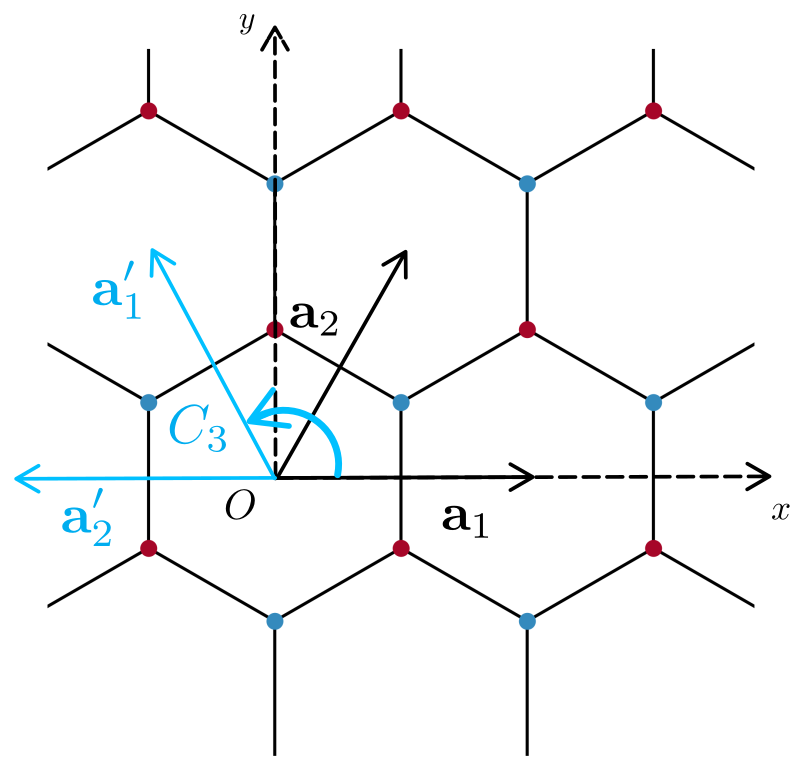
\includegraphics[width=0.32\linewidth]{fig/honeycomb_C3.png}\hfill
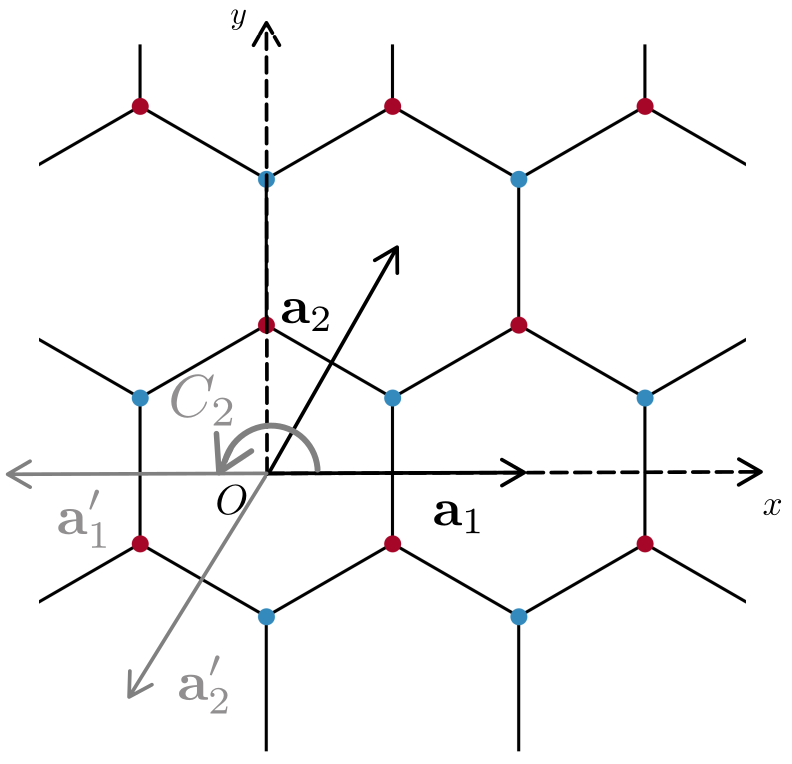
\includegraphics[width=0.32\linewidth]{fig/honeycomb_C2.png}\hfill
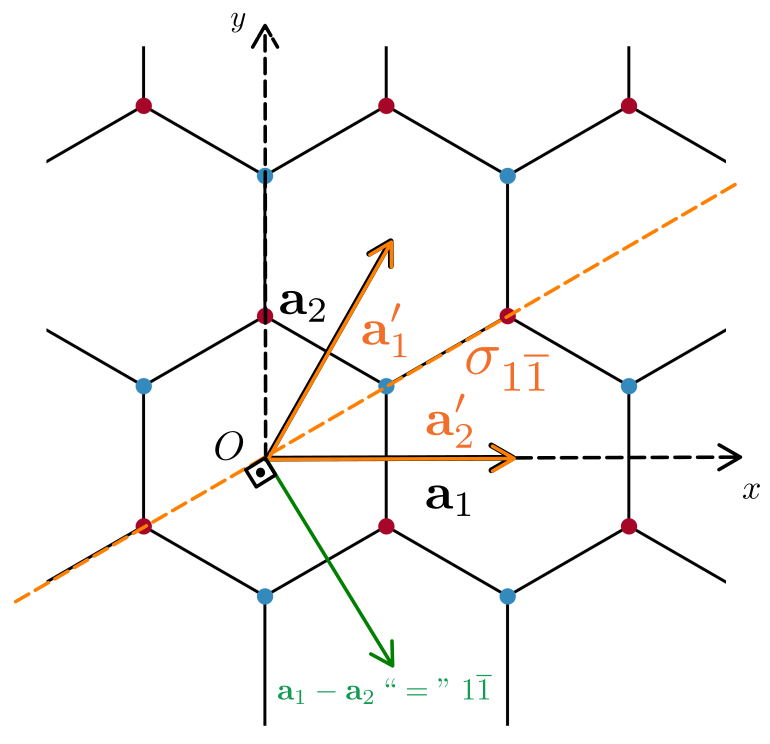
\includegraphics[width=0.32\linewidth]{fig/honeycomb_sigma.png}
\caption{Generators of the point group \(\{C_3, C_2, m_{1\bar{1}}\}\) for the space group \(P6mm\) of the honeycomb lattice, with the coordinate system origin $O$ located at a hexagon's center. \textbf{CORRIGIR} $\sigma_{1\cc{1}} = m_{1\cc{1}}$.}
\label{fig:generators_P6mm}
\end{figure}

Following Figure \ref{fig:generators_P6mm}, we use the basis $\mathcal{B} = \{\a_1 = a \vu{x}, \a_2 = \frac{a}{2} \vu{x} + \frac{a\sqrt{3}}{2} \vu{y}\}$. In this basis, the generators \(\{C_3, C_2, m_{1\bar{1}}\}\) for the point group $6mm$ act like:
\begin{equation} \label{eq:generators_P6mm}
\begin{cases}
\; C_3 \a_1 = -\a_1+\a_2 \\
\; C_3 \a_2 = -\a_1
\end{cases}
\quad
\begin{cases}
\; C_2\a_1 = -\a_1 \\
\; C_2\a_2 = -\a_2
\end{cases}
\quad
\begin{cases}
\; m_{1\bar{1}} \a_1 = \a_2 \\
\; m_{1\bar{1}} \a_2 = \a_1
\end{cases}
\end{equation}

The 6-fold rotation is given by $\{C_6 \mid 0\} = \{C_2 \mid 0\} \{C_3 \mid 0\}^{-1}$, therefore
\begin{equation} \label{eq:C6_rotation_P6mm}
\begin{cases}
\; C_6 \a_1 = \a_2 \\
\; C_6 \a_2 = -\a_1 + \a_2
\end{cases}
\end{equation}

%%%%%%%%%%%%%%%%%%%%%%%%%%%%%%%%%%%%%%%%%%%%%%%%%%%%%%%%%%%%%%%%%%%%%%%%%%%%%%%%%%%%%%%%%%%%%%%%%%
\section{Definitions}
%%%%%%%%%%%%%%%%%%%%%%%%%%%%%%%%%%%%%%%%%%%%%%%%%%%%%%%%%%%%%%%%%%%%%%%%%%%%%%%%%%%%%%%%%%%%%%%%%%


\begin{definition}[\textbf{Orbit}] \label{def:orbit_q}
Given a point \(\q\), the \textit{orbit} of \(\q\) is the set of all points \textbf{within the same unit cell} that are related to \(\q\) by symmetry elements of the space group \(G\), i.e.,
\begin{equation} \label{eq:orbit_of_q}
\text{Orb}(\q) = G \q = \{g \q \mid g \in G\}.
\end{equation}
\end{definition}

\begin{example} \label{ex:orbit_1a2b3c}
In Figure \ref{fig:unitcell_q1q2q3q4q5}, using the basis $\mathcal{B} = \{\a_1, \a_2\}$, consider the points \(\textcolor{red}{\varhexagonblack} = \q_1 = (0,0)\), \(\textcolor{blue}{\mdblksquare} = \q_2 = \qty(\frac{1}{3}, \frac{1}{3})\), \(\textcolor{green}{\bigstar} = \q_3 = \qty(\frac{1}{2}, 0)\), \(\textcolor{magenta}{\varheartsuit} = \q_4 = \qty(\frac{1}{6}, \frac{1}{6})\), and \(\textcolor{orange}{\spadesuit} = \q_5 = \qty(\frac{1}{4}, 0)\).

Note that the unit cell, as shown in Figure \ref{fig:unitcell_limit}, excludes points that are equivalent under translations by Bravais lattice vectors. By applying all symmetry elements of \(G\) to the points \(\q_1, \q_2, \q_3, \q_4, \q_5\) and retaining only those that lie within the same unit cell, the resulting orbits are represented by the symbols \(\textcolor{red}{\varhexagonblack}\), \(\textcolor{blue}{\mdblksquare}\), \(\textcolor{green}{\bigstar}\), \(\textcolor{magenta}{\varheartsuit}\), and \(\textcolor{orange}{\spadesuit}\), as shown in Figure \ref{fig:unitcell_orbitsymbols}.
\end{example}

\begin{figure}[H]
\centering
\begin{subfigure}{.3\textwidth}
  \centering
  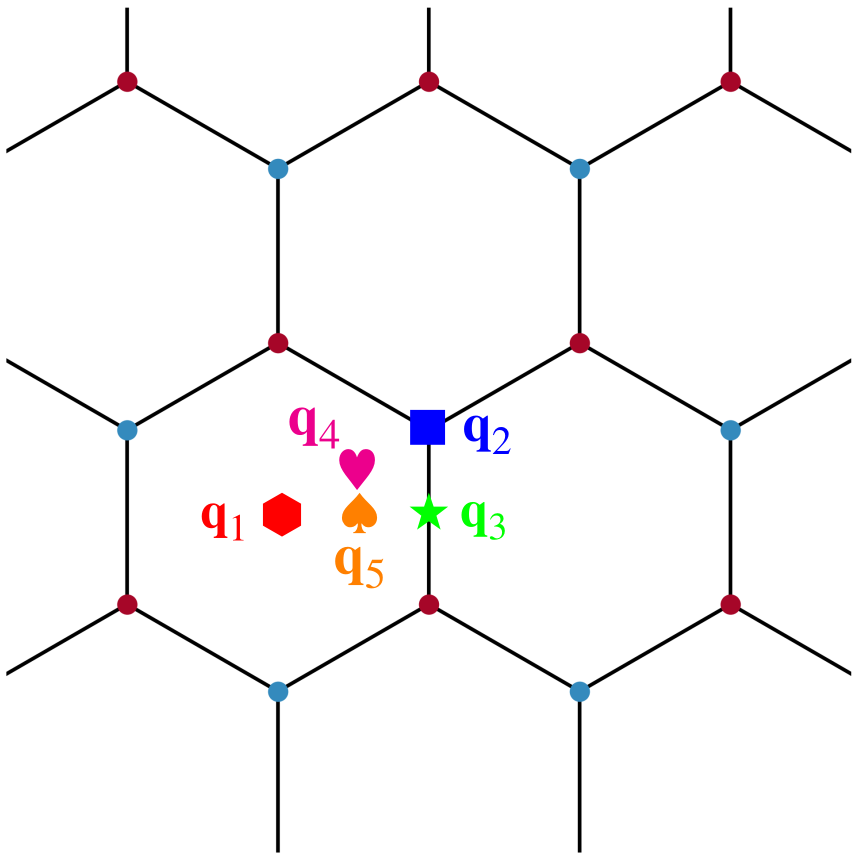
\includegraphics[width=\linewidth]{fig/unitcell_q1q2q3q4q5.png}
  \caption{Points $\q_1,\q_2,\q_3,\q_4,\q_5$}
  \label{fig:unitcell_q1q2q3q4q5}
\end{subfigure}
\hfill
\begin{subfigure}{.3\textwidth}
  \centering
  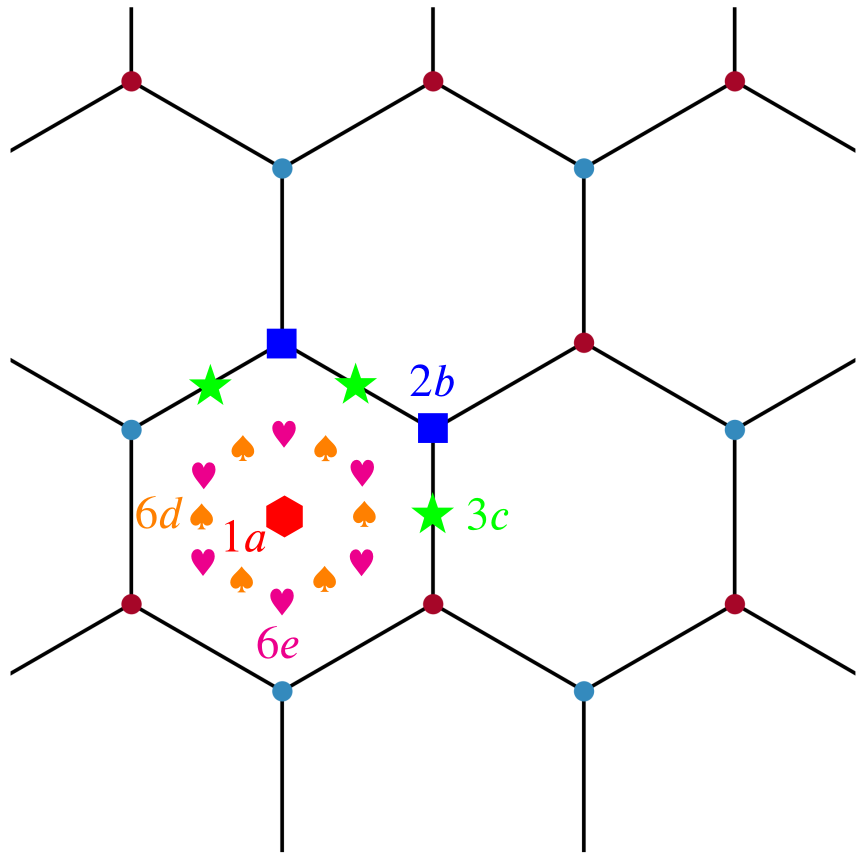
\includegraphics[width=\linewidth]{fig/unitcell_orbitsymbols.png}
  \caption{Orbits and Wyckoff letters}
  \label{fig:unitcell_orbitsymbols}
\end{subfigure}
\hfill
\begin{subfigure}{.235\textwidth}
  \centering
  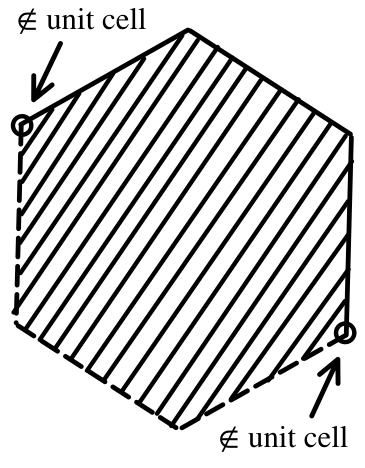
\includegraphics[width=\linewidth]{fig/unitcell_limit.png}
  \caption{Unit cell choice}
  \label{fig:unitcell_limit}
\end{subfigure}
\caption{Unit cell and orbits.}
\label{fig:unitcell_orbits}
\end{figure}


\begin{definition}[\textbf{Site-symmetry group / Stabilizer group}] \label{def:sitesym}
The site-symmetry group of a position $\q$ is the subgroup of operations $g \in G$ that leave $\q$ fixed.
\begin{equation} \label{eq:site-symmetry_def}
G_\q = \{g \mid g \q = \q\} \subseteq G.
\end{equation}
\end{definition}

\textit{Remarks:}
\begin{itemize}
\item The site-symmetry group \( G_\q \) may include elements \(\{R \mid \r\}\) with \(\r \neq \0\).
\item Since any site-symmetry group leaves a point invariant, it is isomorphic to one of the crystallographic point groups: $32$ in three dimensions and $10$ in two dimensions.

\end{itemize}

\begin{example} \label{ex:site-symmetry_groups_p6mm}
Let us identify the site-symmetry groups of points $\q_1$, $\q_2$, $\q_3$, $\q_4$ and $\q_5$.

\begin{itemize}
\item The point $\textcolor{orange}{\spadesuit} = \q_5 = \qty(\frac{1}{4}, 0)$ has a site-symmetry group \(G_{\q_5}\) with only the identity $\{E \mid 0\}$ and $\{m_{x} \mid 0\}$ (reflection by the $x$-axis) as symmetry elements. This makes $G_{\q_5}$ isomorphic to $D_1$.
\begin{equation} \label{eq:site-symmetry-q5}
\{m_{x} \mid 0\} \q_3 = m_x \qty(\frac{1}{4} \a_1) = m_x \qty(\frac{a}{4} \vu{x}) = \frac{a}{4} \vu{x} = \frac{1}{4} \a_1 = \q_5.
\end{equation}


\item The point \(\textcolor{magenta}{\varheartsuit} = \q_4 = \qty(\frac{1}{6}, \frac{1}{6})\) has a site-symmetry group \(G_{\q_4}\) with only the identity $\{E \mid 0\}$ and $\{m_{1\cc{1}} \mid 0\}$ as symmetry elements. This also makes $G_{\q_4}$ isomorphic to $D_1$.
\begin{align} \label{eq:site-symmetry-q4}
\{m_{1\cc{1}} \mid 0\} \q_4 &= m_{1\cc{1}}\qty(\frac{1}{6} \a_1 + \frac{1}{6} \a_2) = \frac{1}{6} \a_2 + \frac{1}{6} \a_1 = \q_4.
\end{align}

\item The point \(\textcolor{green}{\bigstar} = \q_3 = \qty(\frac{1}{2}, 0)\) has a site-symmetry group \(G_{\q_3}\), which is isomorphic to \(D_2\). We can choose its generators to be $\{C_2 \mid \a_1\}$ and $\{m_{x}\mid 0\}$.
\begin{align} \label{eq:site-symmetry-q3}
\{C_2 \mid \a_1\} \q_3 &= C_2 \q_3 + \a_1 = -\q_3 + \a_1 = -\frac{1}{2} \a_1 + \a_1 = \q_3, \\
\{m_{x} \mid 0\} \q_3 &= m_x \qty(\frac{1}{2} \a_1) = m_x \qty(\frac{a}{2} \vu{x}) = \frac{1}{2} \a_1 = \q_3.
\end{align}

\item The point $\textcolor{blue}{\mdblksquare} = \q_2 = \qty(\frac{1}{3}, \frac{1}{3})$ has site-symmetry group $G_{\q_2}$ isomorphic to $D_3$, and its generators are $\{C_3 \mid \a_1\}$ and $\{m_{1\cc{1}} \mid 0\}$.
\begin{align} \label{eq:site-symmetry-q2}
\{C_3 \mid \a_1\} \q_2 &= C_3 \qty(\frac{1}{3} \a_1 + \frac{1}{3} \a_2) + \a_1 = \frac{1}{3} \qty(-2\a_1 + \a_2) + \a_1 =
\frac{1}{3} (\a_1 + \a_2) = \q_2, \\
\{m_{1\cc{1}} \mid 0\} \q_2 &= m_{1\cc{1}} \qty(\frac{1}{3} \a_1 + \frac{1}{3} \a_2) =
\frac{1}{3} \a_2 + \frac{1}{3} \a_1 = \q_2.
\end{align}

\item The point \(\textcolor{red}{\varhexagonblack} = \q_1 = (0,0)\) has a site-symmetry group \(G_{\q_1}\) isomorphic to \(D_6\), with generators \(\{C_3 \mid 0\}\), \(\{C_2 \mid 0\}\), and \(\{m_{1\cc{1}} \mid 0\}\). Since \(\q_1 = \0\) is the origin, it is evident that the action of any generator \(g\) on \(\q_1\) leaves it unchanged:
\begin{equation} \label{eq:site-symmetry-q1}
g \q_1 = \0 = \q_1, \quad \text{for all } g \in G_{\q_1}.
\end{equation}
\end{itemize}

\end{example}

\begin{definition}[\textbf{Wyckoff position}] \label{def:wyckpos}
A \textit{Wyckoff position} \( \q \) refers to any position within the unit cell of the crystal. Some Wyckoff positions are \textit{special}, meaning they are left invariant by certain symmetry operations (other than the identity $\{E \mid 0\}$). The \textit{multiplicity} $n$ of a Wyckoff position is the number of distinct positions in its orbit within the same unit cell, $n = \abs{\text{Orb}(q)}$. A Wyckoff position is generally denoted as \( n\ell \), where \( \ell \) is an alphabetical label that designates the increasing size of the site-symmetry group associated with the position.
\end{definition}

\begin{example} \label{ex:wyckpos_q1q2q3q4q5}
The Wyckoff positions \( \q_1 = \textcolor{red}{\varhexagonblack} \), \( \q_2 = \textcolor{blue}{\mdblksquare} \), \( \q_3 = \textcolor{green}{\bigstar} \), \( \q_4 = \textcolor{magenta}{\varheartsuit} \), and \( \q_5 = \textcolor{orange}{\spadesuit} \) are respectively labeled as \( \textcolor{red}{1a} \), \( \textcolor{blue}{2b} \), \( \textcolor{green}{3c} \), \( \textcolor{magenta}{6d} \), and \( \textcolor{orange}{6e} \), as shown in Figure \ref{fig:unitcell_orbitsymbols}.
\end{example}

\begin{definition}[\textbf{Coset representatives}] \label{def:cosetrep_wyckoff}
The \textit{coset representatives} of the site-symmetry group are the elements \( g_\alpha \) that generate the orbit of a Wyckoff position \( \q \), with each element in the orbit given by \( \q_\alpha = g_\alpha \q \). The number of coset representatives corresponds to the multiplicity of the Wyckoff position.
\end{definition}

\begin{example} \label{ex:coset_representatives_q1q2q3q4q5}
For the points $\q_1 = \textcolor{red}{\varhexagonblack}$, $\q_2 = \textcolor{blue}{\mdblksquare}$, $\q_3 = \textcolor{green}{\bigstar}$, $\q_4 = \textcolor{magenta}{\varheartsuit}$ and $\q_5 = \textcolor{orange}{\spadesuit}$, we can choose coset representatives as
\begin{align}
\text{Orb}(\q_1) &= \qty{\{E\mid 0\} \q_1}, \nonumber \\
                 &= \qty{\qty(0,0)}; \label{eq:orbit_q1} \\
\text{Orb}(\q_2) &= \qty{\{E\mid 0\} \q_2, \{C_6\mid 0\} \q_2}, \label{eq:orbit_q2} \nonumber \\
                 &= \qty{\qty(\frac{1}{3},\frac{1}{3}),\qty(-\frac{1}{3},\frac{2}{3})}; \\
\text{Orb}(\q_3) &= \qty{\{E\mid 0\} \q_3, \{C_6\mid 0\} \q_3, \{C_6^2\mid 0\} \q_3}, \label{eq:orbit_q3} \nonumber \\
                 &= \qty{\qty(\frac{1}{2},0),\qty(0,\frac{1}{2}),\qty(-\frac{1}{2},\frac{1}{2})}; \\
\text{Orb}(\q_4) &= \qty{\{E\mid 0\} \q_4, \{C_6\mid 0\} \q_4, \{C_6^2\mid 0\} \q_4, \{C_6^3\mid 0\} \q_4, \{C_6^4\mid 0\} \q_4, \{C_6^5\mid 0\} \q_4}, \label{eq:orbit_q4} \nonumber \\
                 &= \qty{\qty(\frac{1}{6},\frac{1}{6}),\qty(-\frac{1}{6},\frac{1}{3}),\qty(-\frac{1}{3},\frac{1}{6}),\qty(-\frac{1}{6},-\frac{1}{6}),\qty(\frac{1}{6},-\frac{1}{3}),\qty(\frac{1}{3},-\frac{1}{6})}; \\
\text{Orb}(\q_5) &= \qty{\{E\mid 0\} \q_5, \{C_6\mid 0\} \q_5, \{C_6^2\mid 0\} \q_5, \{C_6^3\mid 0\} \q_5, \{C_6^4\mid 0\} \q_5, \{C_6^5\mid 0\} \q_5}, \label{eq:orbit_q5} \nonumber \\
                 &= \qty{\qty(\frac{1}{4},0),\qty(0,\frac{1}{4}),\qty(-\frac{1}{4},\frac{1}{4}),\qty(-\frac{1}{4},0),\qty(0,-\frac{1}{4}),\qty(\frac{1}{4},-\frac{1}{4})}.
\end{align}
For example, in Equation \ref{eq:orbit_q3}, the coset representatives of $G_{\q_3}$ are $g_1 = \{E\mid 0\}$, $g_2 = \{C_6\mid 0\}$, and $g_3 = \{C_6^2\mid 0\}$.
\end{example}

\begin{lemma}[\textbf{Coset decomposition}] \label{lemma:cosetdecomp_wyckoff}
Let \( \q \) be a Wyckoff position in a space group \( G \). The coset decomposition of \( G \) with respect to \( \q \) is given by:
\begin{equation} \label{eq:coset_decomp_wyckoff}
G = \bigcup_\alpha g_\alpha (G_{\q} \ltimes \Z^d),
\end{equation}
where \( \Z^d \) represents the group of lattice translations, \(\{E\mid \t\}\), with \(\t = \sum_{i=1}^d n_i \a_i\), where \( n_i \in \Z \) and \(\{\a_i\}\) are the primitive lattice vectors in \( d \) dimensions.

In practice, this decomposition means that for any \( g \in G \), we can write \( g = \{E \mid \t\} g_\alpha h \), for some translation \(\t\), coset representative \( g_\alpha \), and \( h \in G_\q \). Applying \( \q \) to both sides:
\begin{equation} \label{eq:coset_decomp_translation_t_step1}
g \q = \{E \mid \t\} g_\alpha h \q = \{E \mid \t\} g_\alpha \q = \{E \mid \t\} \q_\alpha = \q_\alpha + \t,
\end{equation}
which leads to
\begin{equation} \label{eq:coset_decomp_translation_t}
\t = g \q - \q_\alpha.
\end{equation}
\end{lemma}

\begin{lemma}[\textbf{Conjugate site-symmetry groups}] \label{lemma:conjugate_group_G_qalpha}
Positions \(\q\) and \(\q_\alpha\) on the same orbit are connected by the relation \(\q_\alpha = g_\alpha \q\), where \(g_\alpha\) is a coset representative. For \(h \in G_\q\), the following holds:
\begin{equation} \label{eq:conjugate_group_qalpha}
h \q = \q \implies h g_\alpha^{-1} \q_\alpha = g_\alpha^{-1} \q_\alpha \implies
\qty(g_\alpha h g_\alpha^{-1}) \q_\alpha = \q_\alpha \implies
g_\alpha h g_\alpha^{-1} \in G_{\q_\alpha}.
\end{equation}
Consequently, the site-symmetry groups of points on the same orbit are conjugates of each other, satisfying \(G_{\q_\alpha} = g_\alpha G_\q g_\alpha^{-1}\).
\end{lemma}


\begin{definition}[\textbf{Maximal Wyckoff position}] \label{def:maximal_wyckpos}
A site-symmetry group is \textit{non-maximal} if there exists a finite group $H \neq G_\q$, such that $G_\q \subseteq H \subseteq G$. A site-symmetry group that is not non-maximal is \textit{maximal}. A Wyckoff position $\q$ is said to be \textit{maximal} if its site-symmetry group $G_\q$ is maximal.
\end{definition}

\begin{example} \label{ex:maximal_wyckpos_example}
We have $G_{\q_4} \subset G_{\q_2}$ and $G_{\q_5} \subset G_{\q_3}$, therefore $\q_4$ and $\q_5$ are non-maximal Wyckoff positions. On the other hand, the Wyckoff positions $\q_1$, $\q_2$, $\q_3$ are maximal. \textbf{Do I prove this?}
\end{example}

%%%%%%%%%%%%%%%%%%%%%%%%%%%%%%%%%%%%%%%%%%%%%%%%%%%%%%%%%%%%%%%%%%%%%%%%%%%%%%%%%%%%%%%%%%%%%%%%%%
\subsection{Band Representations}
%%%%%%%%%%%%%%%%%%%%%%%%%%%%%%%%%%%%%%%%%%%%%%%%%%%%%%%%%%%%%%%%%%%%%%%%%%%%%%%%%%%%%%%%%%%%%%%%%%

Consider a site \(\q\) within a Wyckoff position of multiplicity \(n\), hosting \(n_q\) orbitals. The corresponding wavefunctions, denoted as \(W_{i1}(\r)\) for \(i = 1, \ldots, n_q\), transform under an \(n_q\)-dimensional representation \(\rho\) of the site-symmetry group \(G_\q\):
\begin{equation} \label{eq:gWi1_nq_rep}
h W_{i1}(\r) = W_{i1}(h^{-1} \r) = \sum_{j} [\rho(h)]_{ij} W_{j1}(\r), \quad h \in G_\q.
\end{equation}

Without loss of generality, let the equivalent sites \(\q_\alpha = g_{\alpha} \q\) be in the same unit cell as \(\q\). The orbitals at \(\q_\alpha\) transform under the conjugate representation \(\rho_\alpha(h) = \rho(g_\alpha^{-1} h g_\alpha)\), where \(h \in G_{\q_\alpha}\) and \(g_\alpha^{-1} h g_\alpha \in G_\q\). The wavefunctions localized at \(\q_\alpha\) are then given by
\begin{equation} \label{eq:Wialpha_galpha_action}
W_{i\alpha}(\r) = g_\alpha W_{i1}(\r) = W_{i1}(g_\alpha^{-1} \r),
\end{equation}
where \(\alpha = 1, \ldots, n\) indexes the equivalent sites that belong to the Wyckoff position of multiplicity \(n\). The wavefunctions on other unit cells are obtained by applying a translation operator, such that:
\begin{equation} \label{eq:translated_Wialpha}
\sg{E}{\t_\mu} W_{i\alpha}(\r) = W_{i\alpha}(\r-\t_\mu),
\end{equation}
where $\t_\mu$ is a Bravais lattice vector.

There are \(n \times n_\q \times N\) wavefunctions \(W_{i\alpha}(\r - \t_\mu)\), where \(N \to \infty\) is the number of unit cells in the system. To determine their transformation properties under an arbitrary space group element \(g = \sg{R}{\t} \in G\), we derive the band representation \(\rho_G = \rho \uparrow G\) induced from the representation \(\rho\) of the site-symmetry group \(G_\q\), as in Definition \ref{def:induction_defi}.
\begin{equation} \label{eq:induced_rho_G_wannier_step1}
\rho_G(g) W_{i\alpha}(\r-\t_\mu) =
\underbrace{g \sg{E}{\t_\mu}}_{= \sg{E}{R\t_\mu} g} W_{i\alpha} (\r) =
\sg{E}{R\t_\mu} g W_{i\alpha} (\r) =
\sg{E}{R\t_\mu} \, (g g_\alpha) \, W_{i1} (\r).
\end{equation}

Applying Lemma \ref{lemma:cosetdecomp_wyckoff} for the element $g g_\alpha \in G$, we write $g g_\alpha = \sg{E}{\t_{\beta\alpha}} g_\beta h$, for some $h \in G_\q$, coset representative $g_\beta$ and a Bravais lattice vector $\t_{\beta\alpha}$ given by
\begin{equation} \label{eq:t_betaalpha}
\t_{\beta\alpha} = gg_\alpha \q - \q_\beta = g \q_\alpha - \q_\beta, \quad
g g_\alpha = \sg{E}{\t_{\beta\alpha}} g_\beta h \implies h = g_\beta^{-1} \{E\mid -\t_{\beta\alpha}\} g g_\alpha.
\end{equation}

Following the derivation from Equation \ref{eq:induced_rho_G_wannier_step1}:
$$
\rho_G(g) W_{i\alpha}(\r-\t_\mu) =
\sg{E}{R\t_\mu} \qty(\sg{E}{\t_{\beta\alpha}} g_\beta h) W_{i1}(\r) =
\sg{E}{R\t_\mu + \t_{\beta\alpha}} g_\beta \sum_{j} [\rho(h)]_{ij} W_{j1}(\r) =
$$
$$
= \sum_{j} \sg{E}{R\t_\mu + \t_{\beta\alpha}} [\rho(h)]_{ij} W_{j\beta}(\r) \implies
$$
\begin{equation} \label{eq:wannier_rep}
\rho_G(g) W_{i\alpha}(\r-\t_\mu) = \sum_{j} [\rho(h)]_{ij} W_{j\beta}(\r - R\t_\mu - \t_{\beta\alpha}).
\end{equation}

\n

Now define the Bloch functions:
\begin{equation} \label{eq:bloch_functions}
a_{i\alpha}(\k, \r) = \sum_{\mu} e^{i\k\vdot\t_\mu} W_{i\alpha}(\r-\t_\mu).
\end{equation}

Using Equation \ref{eq:wannier_rep}, the Bloch functions transform as
$$
\rho_G(g) a_{i\alpha}(\k,\r) =
\rho_G(g) \sum_{\mu} e^{i\k\vdot\t_\mu} W_{i\alpha}(\r-\t_\mu) =
\sum_{j} \sum_{\mu} e^{i\k\vdot\t_\mu} [\rho(h)]_{ij} W_{j\beta}(\r-R\t_\mu-\t_{\beta\alpha}) =
$$
$$
= e^{-i(R\k)\vdot\t_{\beta\alpha}} \sum_{j} [\rho(h)]_{ji} \sum_{\mu} e^{i(R\k)\vdot(R\t_\mu+\t_{\beta\alpha})} W_{j\beta}(\r-R\t_\mu-\t_{\beta\alpha}) \implies
$$
\begin{equation} \label{eq:bloch_rep}
(\rho_G(g) a)_{i\alpha}(\k,\r) = e^{-i(R\k)\vdot\t_{\beta\alpha}} \sum_{j} [\rho(h)]_{ji} \, a_{j\beta}(R\k, \r),
\end{equation}
where $h$ and $\t_{\beta\alpha}$ are determined by Equation \ref{eq:t_betaalpha}. The choice of representatives $g_\alpha$ must be kept fixed through the construction.

Observe that $\rho_G(g)$ in its matrix form consists of infinitely many $(n\cdot n_q)\times (n\cdot n_q)$ block, where each one is labelled by a $(\k', \k)$ pair, that correspond to Bloch functions labelled by $\k', \k$. For a given $g = \sg{R}{\t} \in G$ and each set of columns corresponding to $\k$, there is exactly one non-zero block, identified by $\k' = R\k$. Denoting this block by $\rho_G^\k(g)$, its matrix elements are given by
\begin{equation} \label{eq:k_block_inducedrep_jbia}
\qty[\rho_G^\k(g)]_{j\beta,i\alpha} = e^{-i(R\k)\vdot\t_{\beta\alpha}}\rho_{ji}(g_\beta^{-1}\sg{E}{-\t_{\beta\alpha}}gg_\alpha).
\end{equation}

The full set of matrices $\rho_G^\k(g)$, for each $\k$ in the first BZ, contain all the non-zero elements of $\rho_G(g)$.

%%%%%%%%%%%%%%%%%%%%%%%%%%%%%%%%%%%%%%%%%%%%%%%%%%%%%%%%%%%%%%%%%%%%%%%%%%%%%%%%%%%%%%%%%%%%%%%%%%%
%\subsection{Momentum space}
%%%%%%%%%%%%%%%%%%%%%%%%%%%%%%%%%%%%%%%%%%%%%%%%%%%%%%%%%%%%%%%%%%%%%%%%%%%%%%%%%%%%%%%%%%%%%%%%%%%

\begin{definition}[\textbf{Little group}]
Two reciprocal space vectors $\k_1$ and $\k_2$ are said to be equivalent, $\k_1 \equiv \k_2$, if $\k_2 - \k_1$ is a reciprocal lattice vector. The \textit{little group} $G_\k$ of a vector $\k$ in reciprocal space is the set of elements $g \in G$ such that $g \k \equiv \k$. Remember that the action of space group elements on reciprocal space is defined by
$$
g\k = \sg{R}{\t}\k = R\k.
$$
For each $\k$, notice that $G_\k$ is infinite because if $h \in G_\k$, the operation of $h$ followed by any Bravais lattice translation also belongs to $G_\k$.
\end{definition}

\n

The set \(\{\rho_G^\k(g) \mid g \in G_\k\}\) forms an \((n \cdot n_q) \times (n \cdot n_q)\) representation of the little group \(G_\k\), referred to as \(\rho_G \downarrow G_\k\). This subduction of \(\rho_G\) onto \(G_\k\) is projected onto the Wannier functions at \(\k\). Despite \(G_\k\) being infinite, the representations of two space group operations, \(\sg{R}{\t}\) and \(\sg{R}{\t + \t_1}\), where \(\t_1\) is a Bravais lattice translation, differ only by an overall phase factor \(e^{-i(R\k) \vdot \t_1} = e^{i\k \vdot \t_1}\) within \(\rho_G \downarrow G_\k\).

The characters of \(\rho_G^\k = \rho_G \downarrow G_\k\), analogous to the expression for induced representations' characters, are given for \(g \in G_\k\) as:

\begin{equation} \label{eq:}
\chi^{\rho_G^\k}(g) =
\sum_{\substack{\alpha=1 \\ g_\alpha^{-1}\sg{E}{-\t_{\alpha\alpha}}g g_\alpha \in G_\q}}^n e^{-i(R\k)\vdot\t_{\alpha\alpha}}
\chi^{(\rho)}\qty(g_\alpha^{-1}\sg{E}{-\t_{\alpha\alpha}}g g_\alpha).
\end{equation}

To determine the number of times each irrep \(\sigma_i^\k\) of \(G_\k\) appears in the representation \(\rho_G \downarrow G_\k\), denoted by \(r_i^\k\), we use the decomposition:

\begin{equation} \label{eq:induce_subduce}
(\rho \uparrow G) \downarrow G_\k \equiv \bigoplus_i r_i^\k \sigma_i^\k,
\end{equation}
where \(\equiv\) signifies the equivalence of representations. The multiplicities \(r_i^\k\) are computed using the \textit{Reduction Formula} \ref{eq:reduction_formula}:

%%%%%%%%%%%%%%%%%%%%%%%%%%%%%%%%%%%%%%%%%%%%%%%%%%%%%%%%%%%%%%%%%%%%%%%%%%%%%%%%%%%%%%%%%%%%%%%%%%
\subsection{Spinful Graphene Example} \label{subsec:spinful_graphene}
%%%%%%%%%%%%%%%%%%%%%%%%%%%%%%%%%%%%%%%%%%%%%%%%%%%%%%%%%%%%%%%%%%%%%%%%%%%%%%%%%%%%%%%%%%%%%%%%%%

Let us consider the Wyckoff position 2b on the honeycomb lattice. According to Equation \ref{eq:orbit_q2}, its orbit have the positions with coordinates $\q_2^{(1)} = \qty(\frac{1}{3}, \frac{1}{3})$ e $\q_2^{(2)} = \qty(-\frac{1}{3}, \frac{2}{3})$. The site-symmetry group of $\q_2$ is isomorphic to $D_3$. We will focus on $p_z$ orbitals with spin up $\uparrow$ and down $\downarrow$. Remember that for half-integral angular momentum, a rotation of $2\pi$ gives a minus sign instead of the identity. Because of this, our chosen orbitals will transform accordingly to a double-valued representation of the site-symmetry group $G_{\q_2}$.

As we saw in Example \ref{ex:site-symmetry_groups_p6mm}, the generators for $G_{\q_2}$ can be chosen as $\{C_3 \mid \a_1\}$ and $\{m_{1\cc{1}} \mid 0\}$ in our coordinate system of the honeycomb lattice. For the $p_z$ orbitals with spin up $\uparrow$ and down $\downarrow$, we can choose the matrix representation $\Pi$ according to \cite{building_blocks2018, lectures_tms2017}
\begin{align} \label{eq:site_symmetry_Gq2_SU2_matrixrep}
\Pi\qty(\{C_3 \mid \a_1\}) &= e^{\frac{i \pi}{3} \sigma_z} =
\begin{pmatrix}
e^{\frac{i\pi}{3}} & 0 \\
0 & e^{\frac{-i\pi}{3}}
\end{pmatrix},
\\
\Pi\qty(\{m_{1\cc{1}} \mid 0\}) &= i \sigma_x =
\begin{pmatrix}
0 & i \\
i & 0
\end{pmatrix},
\end{align}
where $\sigma_{x,y,z}$ are the Pauli matrices. Notice that $\Pi\qty(\{m_{1\cc{1}} \mid 0\}) = (i \sigma_x)^2 = -\1 = \Pi\qty(\cc{E})$, because we are dealing with a double group. If we take the trace to compute the characters, we obtain
\begin{equation} \label{eq:characters_doublerep_spinfulgraphene}
\chi^{(\Pi)}\qty(E) = 2, \quad
\chi^{(\Pi)}\qty(\{C_3 \mid \a_1\}) = 1, \quad
\chi^{(\Pi)}\qty(\{m_{1\cc{1}} \mid 0\}) = 0, \quad
\chi^{(\Pi)}\qty(\cc{E}) = -2.
\end{equation}

We see that our site-symmetry group with spinful orbitals is isomorphic to $\cc{D}_3$ and the $\Pi$ representation is actually the irrep $\cc{\Gamma}_6$ from Table \ref{tab:D3_double}.

Let us calculate the induced representation and then subduce it to little groups at high-symmetry points, in other words, compute $(\Pi \uparrow G) \downarrow G_\k$.

First of all, as we have seen in Equation \ref{eq:orbit_q2}, the coset representatives of $G_{\q_2}$ can be chosen $g_1 = \{E \mid 0\}$ and $g_2 = \{C_6 \mid 0\}$. We need to compute $\t_{\beta\alpha}$ for every generator of $G$, which when we exclude translations, can be chosen as $\{C_3\mid 0\}$, $\{m_{1\cc{1}} \mid 0\}$, $\{C_2\mid 0\}$. We decompose $g g_\alpha = \sg{E}{\t_{\beta\alpha}} g_\beta h$ (Equation \ref{eq:t_betaalpha}) for every generator $g$, and we call $\gamma_{\beta\alpha} = g_\beta$ which corresponds to the coset representative $g_\alpha$.

\begin{itemize}
\item $g = \{C_3\mid 0\}$:
\begin{equation} \label{eq:spinful_graphene_generator_C3_g1_induced}
gg_1 = \{C_3 \mid 0\} \{E \mid 0\} = \underbrace{\{E \mid -\a_1\}}_{\{E\mid\t_{11}\}} \underbrace{\{E \mid 0\}}_{g_1 = \gamma_{11}} \underbrace{\{C_3 \mid \a_1\}}_{h_{11}}
\end{equation}
%For $g_2$, we know that the corresponding $g_\beta$ will also be $g_2$, therefore
%\begin{align} \label{eq:spinful_graphene_C3_g2_tbetaalpha_induced}
%\t_{22} &= g \q_2^{(2)} - \q_2^{(2)} = \frac{1}{3} \{C_3 \mid 0\} \qty(-\a_1+2\a_2) - \frac{1}{3} \qty(-\a_1+2\a_2) \\
%&= \frac{1}{3} \qty(-\a_1-\a_2) - \frac{1}{3} \qty(-\a_1+2\a_2) = -\a_2, \\
%h_{22} &= g_2^{-1} \{E \mid -\t_{22}\} g g_2 = \{C_6\mid0\}^{-1}\{E \mid \a_2\}\{C_3\mid 0\} \{C_6 \mid 0\} \\
%&= \{C_6^{-1} \mid 0\} \{C_2 \mid \a_2\} = \{C_6^{-1}C_2 \mid C_6^{-1}\a_2\} = \{C_3 \mid \a_1\}.
%\end{align}
\begin{equation} \label{eq:spinful_graphene_C3_gg2}
gg_2 = \{C_3\mid 0\}\{C_6\mid 0\}= \{E\mid-\a_2\}\{C_2\mid\a_2\}= \underbrace{\{E\mid -\a_2\}}_{\{E\mid \t_{22}\}} \underbrace{\{C_6 \mid 0\}}_{g_2 = \gamma_{22}} \underbrace{\{C_3 \mid \a_1\}}_{h_{22}}.
\end{equation}

From Equation \ref{eq:k_block_inducedrep_jbia}, we have
\begin{align} \label{eq:rhoC3_inducedrep_k_jbia}
\qty[\rho_G^\k(\{C_3\mid0\})]_{j\beta,i\alpha} &=
\begin{pmatrix}
e^{-i(C_3 \k) \vdot \t_{11}} \Pi(h_{11}) & 0 \\
0 & e^{-i(C_3 \k) \vdot \t_{22}} \Pi(h_{22})
\end{pmatrix} \\
&=
\begin{pmatrix}
e^{i(C_3 \k) \vdot \a_1 }\Pi(\{C_3\mid\a_1\}) & 0 \\
0 & e^{i(C_3 \k) \vdot \a_2} \Pi(\{C_3\mid\a_1\})
\end{pmatrix} \\
&=
\begin{pmatrix}
e^{i(C_3 \k) \vdot \a_1} e^{i\frac{\pi}{3} \sigma_z} & 0 \\
0 & e^{i(C_3 \k) \vdot \a_2} e^{i\frac{\pi}{3} \sigma_z}
\end{pmatrix} \\
&=
\begin{pmatrix}
e^{i(C_3 \k) \vdot \a_1} e^{i\frac{\pi}{3}} & 0 & 0 & 0 \\
0 & e^{i(C_3 \k) \vdot \a_1} e^{-i\frac{\pi}{3}} & 0 & 0 \\
0 & 0 & e^{i(C_3 \k) \vdot \a_2} e^{i\frac{\pi}{3}} & 0 \\
0 & 0 & 0 & e^{i(C_3 \k) \vdot \a_2} e^{-i\frac{\pi}{3}} \\
\end{pmatrix}.
\end{align}

\item $\{C_2\mid 0\}$:

\begin{equation} \label{eq:spinful_graphene_generator_C2_g1_induced}
gg_1 = \{C_2 \mid 0\} \{E \mid 0\} = \{E\mid-\a_2\} \{C_2 \mid \a_2\} = \underbrace{\{E \mid -\a_2\}}_{\{E\mid\t_{21}\}} \underbrace{\{C_6 \mid 0\}}_{g_2 = \gamma_{21}} \underbrace{\{C_3 \mid \a_1\}}_{h_{21}}
\end{equation}

\begin{equation} \label{eq:spinful_graphene_C2_gg2}
gg_2 = \{C_2\mid 0\}\{C_6\mid 0\}= \{C_3^2\mid0\} = \{E\mid-\a_2\}\{C_3^2\mid\a_2\} = \underbrace{\{E\mid -\a_2\}}_{\{E\mid \t_{12}\}} \underbrace{\{E \mid 0\}}_{g_1 = \gamma_{12}} \underbrace{\{C_3 \mid \a_1\}^2}_{h_{12}}.
\end{equation}

\begin{align} \label{eq:rhoC2_inducedrep_k_jbia}
\qty[\rho_G^\k(\{C_2\mid0\})]_{j\beta,i\alpha} &=
\begin{pmatrix}
0 & e^{-i(C_2 \k) \vdot \t_{12}} \Pi(h_{12}) \\
e^{-i(C_2 \k) \vdot \t_{21}} \Pi(h_{21}) & 0
\end{pmatrix} \\
&=
\begin{pmatrix}
0 & e^{i(C_2 \k) \vdot \a_2} \Pi(\{C_3\mid\a_1\})^2 \\
e^{i(C_2 \k) \vdot \a_2} \Pi(\{C_3\mid\a_1\}) & 0
\end{pmatrix} \\
&=
\begin{pmatrix}
0 & e^{i(C_2 \k) \vdot \a_2} e^{i\frac{\pi}{3} \sigma_z^2} \\
e^{i(C_2 \k) \vdot \a_2} e^{i\frac{\pi}{3} \sigma_z} & 0
\end{pmatrix} \\
&=
\begin{pmatrix}
0 & 0 & e^{i(C_2 \k) \vdot \a_2} e^{i\frac{\pi}{3}} & 0 \\
0 & 0 & 0 & e^{i(C_2 \k) \vdot \a_2} e^{i\frac{\pi}{3}} \\
e^{i(C_2 \k) \vdot \a_2} e^{i\frac{\pi}{3}} & 0 & 0 & 0 \\
0 & e^{i(C_2 \k) \vdot \a_2} e^{-i\frac{\pi}{3}} & 0 & 0 \\
\end{pmatrix}.
\end{align}


\item $g = \{C_6 \mid 0\}$:

\begin{equation} \label{eq:spinful_graphene_generator_C6_g1_decomp}
gg_1 = \{C_6 \mid 0\} \{E \mid 0\} = \underbrace{\{E \mid 0\}}_{\{E\mid\t_{21}\}} \underbrace{\{C_6 \mid 0\}}_{g_2 = \gamma_{21}} \underbrace{\{E \mid 0\}}_{h_{21}}
\end{equation}
\begin{equation} \label{eq:spinful_graphene_generator_C6_g2_decomp}
gg_2 = \{C_6 \mid 0\} \{C_6 \mid 0\} = \{C_3 \mid 0\} =  \underbrace{\{E \mid -\a_1\}}_{\{E\mid\t_{12}\}} \underbrace{\{E \mid 0\}}_{g_1 = \gamma_{12}} \underbrace{\{C_3 \mid \a_1\}}_{h_{12}}
\end{equation}

\begin{align} \label{eq:rhoC6_inducedrep_k_jbia}
\qty[\rho_G^\k(\{C_6\mid0\})]_{j\beta,i\alpha} &=
\begin{pmatrix}
0 & e^{-i(C_6 \k) \vdot \t_{12}} \Pi(h_{12}) \\
e^{-i(C_6 \k) \vdot \t_{21}} \Pi(h_{21}) & 0
\end{pmatrix} \\
&=
\begin{pmatrix}
0 & e^{i (C_6 \k) \vdot \a_1} \Pi(\{C_3 \mid \a_1\}) \\
\Pi(E) & 0
\end{pmatrix} \\
&=
\begin{pmatrix}
0 & e^{i (C_6 \k) \vdot \a_1} e^{i\frac{\pi}{3}\sigma_z} \\
\1 & 0
\end{pmatrix} \\
&=
\begin{pmatrix}
0 & 0 & e^{i (C_6 \k) \vdot \a_1} e^{\frac{i\pi}{3}} & 0 \\
0 & 0 & 0 & e^{i (C_6 \k) \vdot \a_1} e^{-\frac{i\pi}{3}} \\
1 & 0 & 0 & 0 \\
0 & 1 & 0 & 0 \\
\end{pmatrix}.
\end{align}

%Since $\{C_3\mid 0\} = \{C_6\mid 0\}^2$, we can multiply \ref{eq:rhoC6_inducedrep_k_jbia} by itself to obtain
%\begin{equation} \label{eq:rhoC3_jbia_matrix}
%\qty[\rho_G^\k(\{C_3\mid0\})]_{j\beta,i\alpha} =
%\begin{pmatrix}
%e^{i (C_6 \k) \vdot \a_1} e^{\frac{i\pi}{3}} & 0  & 0 & 0 \\
%0 & e^{i (C_6 \k) \vdot \a_1} e^{-\frac{i\pi}{3}} & 0 & 0 \\
%0 & 0 & e^{i (C_6 \k) \vdot \a_1} e^{\frac{i\pi}{3}} & 0  \\
%0 & 0 & 0 & e^{i (C_6 \k) \vdot \a_1} e^{-\frac{i\pi}{3}} \\
%\end{pmatrix}
%\end{equation}
%
%For $\{C_2 \mid 0\} = \{C_6\mid 0\}^3$, we have
%\begin{equation} \label{eq:rhoC2_jbia_matrix}
%\qty[\rho_G^\k(\{C_2\mid0\})]_{j\beta,i\alpha} =
%\begin{pmatrix}
%0 & 0 & e^{2 i (C_6 \k) \vdot \a_1} e^{\frac{2\pi i}{3}} & 0  \\
%0 & 0 & 0 & e^{2 i (C_6 \k) \vdot \a_1} e^{-\frac{2\pi i}{3}} \\
%e^{i (C_6 \k) \vdot \a_1} e^{\frac{i\pi}{3}} & 0  & 0 & 0 \\
%0 & e^{i (C_6 \k) \vdot \a_1} e^{-\frac{i\pi}{3}} & 0 & 0 \\
%\end{pmatrix}
%\end{equation}


\item $\{m_{1\cc{1}} \mid 0\}$:

\begin{equation} \label{eq:spinful_graphene_generator_C6_g1_decomp}
gg_1 = \{m_{1\cc{1}} \mid 0\} \{E \mid 0\} = \underbrace{\{E \mid 0\}}_{\{E\mid\t_{11}\}} \underbrace{\{E \mid 0\}}_{g_1 = \gamma_{11}} \underbrace{\{m_{1\cc{1}} \mid 0\}}_{h_{11}}
\end{equation}
\begin{equation} \label{eq:spinful_graphene_generator_C6_g2_decomp}
gg_2 = \{m_{1\cc{1}} \mid 0\} \{C_6 \mid 0\} = \underbrace{\{E \mid \a_1-\a_2\}}_{\{E\mid \t_{22}\}} \underbrace{\{C_6\mid 0\}}_{g_2 = \gamma_{22}} \underbrace{\{ m_{1\cc{1}} \mid 0 \} \{C_3\mid\a_1\}}_{h_{22}},
\end{equation}
where we calculated $\t_{22}$ and $h_{22}$ from
$$
\t_{22} = g \q_2^{(2)} - \q_2^{(2)} = \{m_{1\cc{1}} \mid 0\} \q_2^{(2)} - \q_2^{(2)} = \a_1-\a_2
$$
\begin{align} \label{eq:spinful_graphene_generator_C6_g2_decomp_h}
h_{22} &= \{C_6^{-1}\mid 0\} \{E \mid -\a_1+\a_2\} \{m_{1\cc{1}} \mid 0\} \{C_6 \mid 0\} =
\{C_6^{-1} \mid \a_2 \}\{m_{1\cc{1}} C_6 \mid 0\} = \\
&= \{C_6^{-1} m_{1\cc{1}} C_6 \mid \a_2\} = \{ m_{1\cc{1}} C_3 \mid \a_2 \} = \{ m_{1\cc{1}} \mid 0 \} \{C_3\mid\a_1\} \in G_{\q_2}.
\end{align}

From Equation \ref{eq:k_block_inducedrep_jbia}, we have
\begin{align} \label{eq:rho_m11_inducedrep_k_jbia}
\qty[\rho_G^\k(\{m_{1\cc{1}}\mid0\})]_{j\beta,i\alpha} &=
\begin{pmatrix}
e^{-i(m_{1\cc{1}} \k) \vdot \t_{11}} \Pi(h_{11}) & 0 \\
0 & e^{-i(m_{1\cc{1}} \k) \vdot \t_{22}} \Pi(h_{22})
\end{pmatrix} \\
&=
\begin{pmatrix}
\Pi(\{m_{1\cc{1}}\mid0\}) & 0 \\
0 & e^{-i(m_{1\cc{1}} \k) \vdot (\a_1-\a_2)} \Pi(\{m_{1\cc{1}}\mid0\}) \Pi(\{C_3\mid \a_1\})
\end{pmatrix} \\
&=
\begin{pmatrix}
i \sigma_x & 0 \\
0 & e^{-i(m_{1\cc{1}} \k) \vdot (\a_1-\a_2)} i \sigma_x e^{i\frac{\pi}{3}\sigma_z}
\end{pmatrix} \\
&=
\begin{pmatrix}
0 & i & 0 & 0 \\
i & 0 & 0 & 0 \\
0 & 0 & 0 & e^{-i(m_{1\cc{1}} \k) \vdot (\a_1-\a_2)} i e^{-\frac{i\pi}{3}} \\
0 & 0 & e^{-i(m_{1\cc{1}} \k) \vdot (\a_1-\a_2)} i e^{ \frac{i\pi}{3}} & 0 \\
\end{pmatrix}.
\end{align}

\end{itemize}

\begin{figure}[H]
\centering
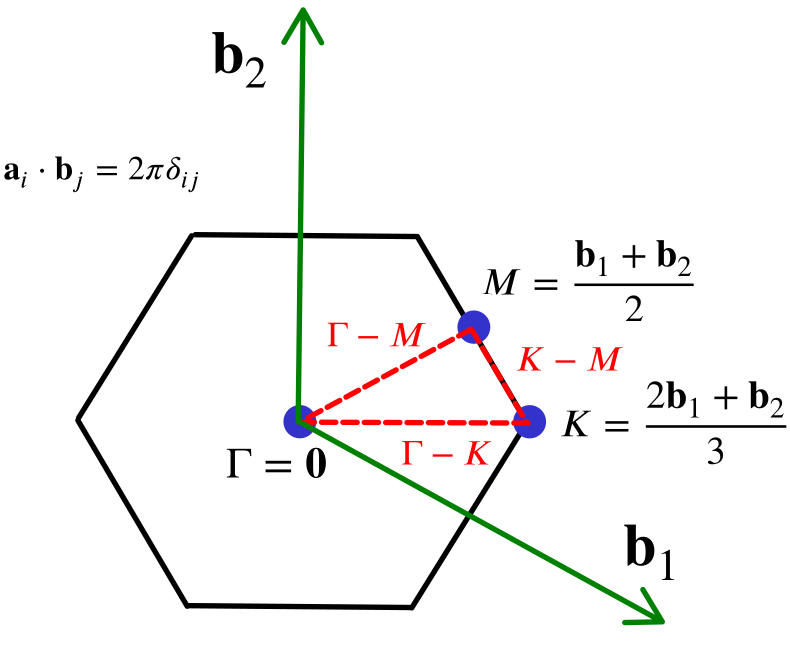
\includegraphics[width=0.6\linewidth]{fig/honeycomb_tqc_BZ.png}
\caption{Brillouin Zone of the honeycomb lattice of Figure \ref{fig:generators_P6mm}, where the momentum lattice vectors $\b_{1,2}$ satisfy $\vb{a}_i \vdot \vb{b}_j = 2\pi \delta_{ij}$.}
\label{fig:honeycomb_tqc_BZ}
\end{figure}


The characters are (if $g \in G_\k$, then $g \k \equiv \k$)
\begin{align} \label{eq:characters_rho_inducedrep_k}
\begin{cases}
\chi^{\rho_G^\k}(\{E\mid 0\}) &= 4, \\
\chi^{\rho_G^\k}(\{C_6\mid 0\}) &= 0, \\
\chi^{\rho_G^\k}(\{C_3\mid 0\}) &= e^{i \k \vdot \a_1} + e^{i \k \vdot \a_2}, \\
\chi^{\rho_G^\k}(\{C_2\mid 0\}) &= 0, \\
\chi^{\rho_G^\k}(\{m_{1\cc{1}}\mid 0\}) &= 0.
\end{cases}
\end{align}

For $\k = \Gamma = \0$ and $\k = K = \frac{2\b_1 + \b_2}{3}$ we have
\begin{equation} \label{eq:characters_rhoC3_k_Gamma_K}
\chi^{\rho_G^\Gamma}(\{C_3\mid 0\}) = 2, \quad
\chi^{\rho_G^K}(\{C_3\mid 0\}) = e^{\frac{2\pi i}{3}} + e^{-\frac{2\pi i}{3}} = -1. \quad
\end{equation}

Notice that $\chi^{\rho_G^M}(\{C_3\mid 0\})$ does not make sense, because $\{C_3\mid 0\} \notin G_M$.

\n

We compare the characters in Equation \ref{eq:characters_rho_inducedrep_k} to the character tables \ref{tab:D6_double}, \ref{tab:D3_double_littlegroup_K} and \ref{tab:D2_double}, in order to discover the multiplicities in Equation \ref{eq:induce_subduce}.

For $\Gamma$, comparison with Table \ref{tab:D6_double} shows that $\rho_G^{\Gamma} = \cc{\Gamma}_8 \oplus \cc{\Gamma}_9$.

\begin{table}[H]
\caption{Character table of group $\cc{D}_6$ (or $\cc{C}_{6v}$).}
\centering
\begin{tabular} { c c c c c c c c c c  }
\specialrule{0.05em}{0em}{0.2em}
$\P$ & $\P E$ & $\P 2 C_3$ & $\P2C_2$ & $\P2C_6$ & $\P6 m$ & $\P6 C_6 m$ & $\cc{E}$ & $2 \cc{C}_3$ & $2 \cc{C}_6$ \\
\specialrule{0.01em}{0.2em}{0.2em}
$\Gamma_1$      & $\P1$ & $\P1$ & $\P1$ & $\P1$ & $\P1$ & $\P1$ & $\P1$ & $\P1$ & $\P1$ \\
\specialrule{0.01em}{0.2em}{0.2em}
$\Gamma_2$      & $\P1$ & $\P1$ & $\P1$ & $\P1$ & $ -1$ & $ -1$ & $\P1$ & $\P1$ & $\P1$ \\
\specialrule{0.01em}{0.2em}{0.2em}
$\Gamma_3$      & $\P1$ & $\P1$ & $ -1$ & $ -1$ & $ -1$ & $\P1$ & $\P1$ & $\P1$ & $ -1$ \\
\specialrule{0.01em}{0.2em}{0.2em}
$\Gamma_4$      & $\P1$ & $\P1$ & $ -1$ & $ -1$ & $\P1$ & $ -1$ & $\P1$ & $\P1$ & $ -1$ \\
\specialrule{0.01em}{0.2em}{0.2em}
$\Gamma_5$      & $\P2$ & $ -1$ & $\P2$ & $ -1$ & $\P0$ & $\P0$ & $\P2$ & $ -1$ & $ -1$ \\
\specialrule{0.01em}{0.2em}{0.2em}
$\Gamma_6$      & $\P2$ & $ -1$ & $ -2$ & $\P1$ & $\P0$ & $\P0$ & $\P2$ & $ -1$ & $\P1$ \\
\specialrule{0.01em}{0.2em}{0.2em}
$\cc{\Gamma}_7$ & $\P2$ & $ -2$ & $\P0$ & $\P0$ & $\P0$ & $\P0$ & $ -2$ & $\P2$ & $\P0$ \\
\specialrule{0.01em}{0.2em}{0.2em}
$\cc{\Gamma}_8$ & $\P2$ & $\P1$ & $\P0$ & $-\sqrt{3}$ & $\P0$ & $\P0$ & $ -2$ & $ -1$ & $\P\sqrt{3}$ \\
\specialrule{0.01em}{0.2em}{0.2em}
$\cc{\Gamma}_9$ & $\P2$ & $\P1$ & $\P0$ & $\P\sqrt{3}$ & $\P0$ & $\P0$ & $ -2$ & $ -1$ & $-\sqrt{3}$ \\
\specialrule{0.01em}{0.2em}{0.2em}
$\rho_G^\Gamma = \cc{\Gamma}_8 \oplus \cc{\Gamma}_9$ & $\P4$ & $\P2$ & $\P0$ & $\P0$ & $\P0$ & $\P0$ & $ -4$ & $ -2$ & $\P0$ \\
\specialrule{0.05em}{0.2em}{0em}
\end{tabular}
\label{tab:D6_double}
\end{table}


For $K$, comparison with Table \ref{tab:D3_double_littlegroup_K} shows that $\rho_G^{K} = \cc{K}_4 \oplus \cc{K}_5 \oplus \cc{K}_6$, where we renamed $\cc{\Gamma}_{4,5,6}$ (in character tables of an abstract group) to $\cc{K}_{4,5,6}$, in order to emphasize the little group at $K$.

\begin{table}[H]
\caption{Character table of double group $\cc{D}_3$ (or $\cc{C}_{3v}$).}
\centering
\begin{tabular} { c c c c c c c  }
\specialrule{0.05em}{0em}{0.2em}
$\P$ & $\P E$ & $\P 2 C_3$ & $\P 3 m$ & $\P \cc{E}$ & $\P 2 \cc{C}_3$ & $\P3\cc{m}$ \\
\specialrule{0.01em}{0.2em}{0.2em}
$K_1$      & $\P1$ & $\P1$ & $\P1$  & $\P1$ & $\P1$ & $\P1$  \\
\specialrule{0.01em}{0.2em}{0.2em}
$K_2$      & $\P1$ & $\P1$ & $ -1$  & $\P1$ & $\P1$ & $ -1$  \\
\specialrule{0.01em}{0.2em}{0.2em}
$K_3$      & $\P2$ & $ -1$ & $\P0$  & $\P2$ & $ -1$ & $\P0$  \\
\specialrule{0.01em}{0.2em}{0.2em}
$\cc{K}_4$ & $\P1$ & $ -1$ & $  -i$ & $ -1$ & $\P1$ & $\P i$  \\
\specialrule{0.01em}{0.2em}{0.2em}
$\cc{K}_5$ & $\P1$ & $ -1$ & $\P i$ & $ -1$ & $\P1$ & $  -i$ \\
\specialrule{0.01em}{0.2em}{0.2em}
$\cc{K}_6$ & $\P2$ & $\P1$ & $\P0$  & $ -2$ & $ -1$ & $\P0$  \\
\specialrule{0.01em}{0.2em}{0.2em}
$\rho_G^{K} = \cc{K}_4 \oplus \cc{K}_5 \oplus \cc{K}_6$    & $\P4$ & $ -1$ & $\P0$  & $ -4$ & $\P1$ & $\P0$  \\
\specialrule{0.05em}{0.2em}{0em}
\end{tabular}
\label{tab:D3_double_littlegroup_K}
\end{table}


For $M$, comparison with Table \ref{tab:D2_double} shows that $\rho_G^M = \cc{M}_5 \oplus \cc{M}_5$. Again, we use $\cc{\Gamma}_5$ to refer to the irrep of the abstract group $\cc{D}_2$, but the notation $\cc{M}_5$ to refer to the irrep of the little group at $M$.

\begin{table}[H]
\caption{Character table of double group $\cc{D}_2$ (or $\cc{C}_{2v}$).}
\centering
\begin{tabular} { c c c c c c }
\specialrule{0.05em}{0em}{0.2em}
$\P$ & $\P E$ & $\P 2 C_2$ & $\P 2 m$ & $\P 2 C_2 m$ & $\P \cc{E}$ \\
\specialrule{0.01em}{0.2em}{0.2em}
$M_1$      & $\P1$ & $\P1$ & $\P1$ & $\P1$ & $\P1$ \\
\specialrule{0.01em}{0.2em}{0.2em}
$M_2$      & $\P1$ & $\P1$ & $ -1$ & $ -1$ & $\P1$ \\
\specialrule{0.01em}{0.2em}{0.2em}
$M_3$      & $\P1$ & $ -1$ & $ -1$ & $\P1$ & $\P1$ \\
\specialrule{0.01em}{0.2em}{0.2em}
$M_4$      & $\P1$ & $ -1$ & $\P1$ & $ -1$ & $\P1$ \\
\specialrule{0.01em}{0.2em}{0.2em}
$\cc{M}_5$ & $\P2$ & $\P0$ & $\P0$ & $\P0$ & $ -2$ \\
\specialrule{0.01em}{0.2em}{0.2em}
$\rho_G^{M} = 2 \cc{M}_5$    & $\P4$ & $\P0$ & $\P0$ & $\P0$ & $ -4$ \\
\specialrule{0.05em}{0.2em}{0em}
\end{tabular}
\label{tab:D2_double}
\end{table}


At each high-symmetry point $(\Gamma, K, M)$, we will decompose the little group irreps that appear at that point into a sum of irreps of the little group of each high-symmetry line emanating from that point. There are three high-symmetry lines: $\Gamma-K$, $\Gamma-M$ and $K-M$. Although the little group of each line is distinct, all three groups are isomorphic to $C_s \ltimes \mathbb{Z}^2$, generated by a single mirror and two primitive lattice translations. Its character table is

\begin{table}[H]
\caption{Character table of double group $\cc{C}_s$.}
\centering
\begin{tabular} { c c c c c }
\specialrule{0.05em}{0em}{0.2em}
$\P$ & $\P E$ & $\P m$ & $\P \cc{E}$ & $\P \cc{m}$ \\
\specialrule{0.01em}{0.2em}{0.2em}
$\Lambda_1$      & $\P1$ & $\P1$ & $\P1$ & $\P1$ \\
\specialrule{0.01em}{0.2em}{0.2em}
$\Lambda_2$      & $\P1$ & $ -1$ & $\P1$ & $ -1$ \\
\specialrule{0.01em}{0.2em}{0.2em}
$\cc{\Lambda}_3$ & $\P1$ & $ -i$ & $ -1$ & $\P i$ \\
\specialrule{0.01em}{0.2em}{0.2em}
$\cc{\Lambda}_4$ & $\P1$ & $\P i$ & $ -1$ & $ -i$ \\
\specialrule{0.05em}{0.2em}{0em}
\end{tabular}
\label{tab:Cs_double}
\end{table}

We are going to call the irreps of the little groups $G_\k$ points of high-symmetry lines $\Lambda_{1,2}$ and $\cc{\Lambda}_{3,4}$. We subduce the groups $G_\Gamma$, $G_K$ and $G_M$ (isomorphic to $\cc{D}_6$, $\cc{D}_3$ and $\cc{D}_2$) to the little group $G_\k$ at high-symmetry lines (isomorphic to $\cc{C}_s$, which is a subgroup of $\cc{D}_6$, $\cc{D}_3$ and $\cc{D}_2$). For this, we compare the representations of the subduction in Table \ref{Cs_subduction_highsymmlines}.

\begin{table}[H]
\caption{Double-valued representations of $\cc{C}_s$ and comparison with subduced representations of $G_\Gamma$, $G_K$ and $G_M$.}
\centering
\begin{tabular} { c c c c c }
\specialrule{0.05em}{0em}{0.2em}
$\P$ & $\P E$ & $\P m$ & $\P \cc{E}$ & $\P \cc{m}$ \\
\specialrule{0.01em}{0.2em}{0.2em}
$\cc{\Lambda}_3$ & $\P1$ & $ -i$ & $ -1$ & $\P i$ \\
\specialrule{0.01em}{0.2em}{0.2em}
$\cc{\Lambda}_4$ & $\P1$ & $\P i$ & $ -1$ & $ -i$ \\
\specialrule{0.01em}{0.2em}{0.2em}
$\cc{\Gamma}_8 \downarrow G_\Lambda \equiv \cc{\Lambda}_3 \oplus \cc{\Lambda}_4$ & $\P2$ & $\P0$ & $ -2$ & $\P0$ \\
\specialrule{0.01em}{0.2em}{0.2em}
$\cc{\Gamma}_9 \downarrow G_\Lambda \equiv \cc{\Lambda}_3 \oplus \cc{\Lambda}_4$ & $\P2$ & $\P0$ & $ -2$ & $\P0$ \\
\specialrule{0.01em}{0.2em}{0.2em}
$\cc{K}_4 \downarrow G_\Lambda \equiv \cc{\Lambda}_3$ & $\P1$ & $  -i$ & $ -1$ & $\P i$  \\
\specialrule{0.01em}{0.2em}{0.2em}
$\cc{K}_5 \downarrow G_\Lambda \equiv \cc{\Lambda}_4$ & $\P1$ & $\P i$ & $ -1$ & $  -i$ \\
\specialrule{0.01em}{0.2em}{0.2em}
$\cc{K}_6 \downarrow G_\Lambda \equiv \cc{\Lambda}_3 \oplus \cc{\Lambda}_4$ & $\P2$ & $\P0$  & $ -2$ & $\P0$  \\
\specialrule{0.01em}{0.2em}{0.2em}
$\cc{M}_5 \downarrow G_\Lambda \equiv \cc{\Lambda}_3 \oplus \cc{\Lambda}_4$ & $\P2$ & $\P0$ & $ -2$ & $\P0$ \\
\specialrule{0.05em}{0.2em}{0em}
\end{tabular}
\label{tab:Cs_double}
\end{table}

With the information about the decomposition of representations of Table \ref{tab:Cs_double}, we can sketch the band structure that respect the representations along the high-symmetry lines. A band that comes from a $\cc{\Lambda}_3$ which arrives at the $K$ point, has to arrive at also a $\cc{\Lambda}_3$ representation, so it can be $\cc{K}_4 \equiv \cc{\Lambda}_3$ or $\cc{K}_6 \equiv \cc{\Lambda}_3 \oplus \cc{\Lambda}_4$, but cannot arrive at $\cc{K}_5 \equiv \cc{\Lambda}_4$. With this restriction in mind, there are only two possible kinds of band structures, which depend on height of the energies, which group theory does not tell us.

\begin{figure}[H]
\centering
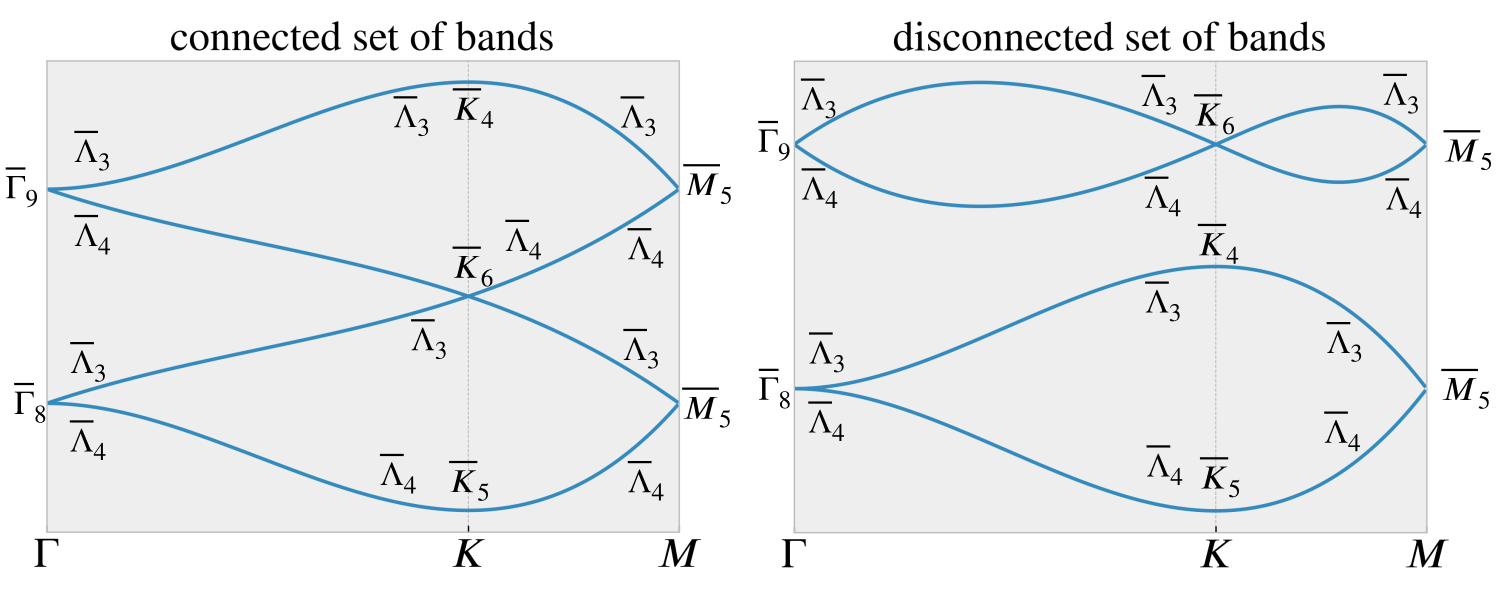
\includegraphics[width=\linewidth]{fig/bands_con_discon.png}
\caption{The two possible kinds of bands from Wyckoff position $2b$.}
\label{fig:bands_con_discon}
\end{figure}








%%%%%%%%%%%%%%%%%%%%%%%%%%%%%%%%%%%%%%%%%%%%%%%%%%%%%%%%%%%%%%%%%%%%%%%%%%%%%%%%%%%%%%%%%%%%%%%%%%
\subsection{Elementary Band Representations}
%%%%%%%%%%%%%%%%%%%%%%%%%%%%%%%%%%%%%%%%%%%%%%%%%%%%%%%%%%%%%%%%%%%%%%%%%%%%%%%%%%%%%%%%%%%%%%%%%%

Two band representations are considered equivalent if they can be continuously deformed into each other without closing energy gaps or breaking symmetries, similar to the concept of homotopy in topology. This notion of equivalence is essential for classifying electronic band structures in terms of their topological properties. By treating equivalence in this way, we can systematically identify whether a material exhibits non-trivial topological phases, such as those found in topological insulators, based purely on its symmetry and band structure.

\begin{definition}[\textbf{Equivalence between band representations}] \label{def:equiv_bandrep}
Two band representations $\rho_G$ and $\sigma_G$ are equivalent iff there exists a unitary matrix-valued function $S(\k,t,g)$ smooth in $\k$ and continuous in $t$ such that, for all $g \in G$
\begin{enumerate}
\item $S(\k, t, g)$ defines a band representation according to Equation \ref{eq:bloch_rep} for all $t \in [0,1]$;
\item $S(\k, 0, g) = \rho_G^\k(g)$;
\item $S(\k, 1, g) = \sigma_G^\k(g)$.
\end{enumerate}
\end{definition}

\begin{definition}[\textbf{Elementary band representation}]
A band representation is called \textbf{composite} if it is equivalent to the direct sum of other band representations. A band representation that is not composite is called \textbf{elementary}.
\end{definition}

%\begin{theorem}[\textbf{Properties of band representations}]
%Some properties of band representations are:
%\begin{enumerate}
%\item Because induction commutes with direct sums
%$$
%(\rho_1 \oplus \rho_2) \uparrow G = (\rho_1 \uparrow G) \oplus (\rho_2 \uparrow G),
%$$
%reducible representations of $G_\q$ induce composite band representations.
%
%\item Given subgroups $K \subset H \subset G$, and a representation $\rho$ of $K$, because induction is transitive it follows that
%$$
%(\rho \uparrow H) \uparrow G = \rho \uparrow G.
%$$
%From this we conclude that all EBRs can be induced from irreps of the maximal site symmetry groups.
%\end{enumerate}
%\end{theorem}

%%%%%%%%%%%%%%%%%%%%%%%%%%%%%%%%%%%%%%%%%%%%%%%%%%%%%%%%%%%%%%%%%%%%%%%%%%%%%%%%%%%%%%%%%%%%%%%%%%%
%\subsection{Exceptions}
%%%%%%%%%%%%%%%%%%%%%%%%%%%%%%%%%%%%%%%%%%%%%%%%%%%%%%%%%%%%%%%%%%%%%%%%%%%%%%%%%%%%%%%%%%%%%%%%%%%
%
%There are exceptions where an irrep of the site symmetry group of a maximal Wyckoff position induces a composite band representation.

%%%%%%%%%%%%%%%%%%%%%%%%%%%%%%%%%%%%%%%%%%%%%%%%%%%%%%%%%%%%%%%%%%%%%%%%%%%%%%%%%%%%%%%%%%%%%%%%%%
\subsection{Topological Systems}
%%%%%%%%%%%%%%%%%%%%%%%%%%%%%%%%%%%%%%%%%%%%%%%%%%%%%%%%%%%%%%%%%%%%%%%%%%%%%%%%%%%%%%%%%%%%%%%%%%

The \textit{atomic limit} refers to bands that can be constructed from localized orbitals situated on atomic sites while fully preserving the crystal's symmetry. These bands represent tightly bound electrons and lack any global topological properties. In contrast, \textit{topological bands} cannot be derived from such localized orbitals without violating symmetry or continuity. Their wavefunctions exhibit a global ``twisting'' that fundamentally sets them apart from the atomic case. Based on this concept, we define the following \cite{building_blocks2018}:

\begin{definition}[\textbf{Topological band}]
A set of bands are in the \textbf{atomic limit} of a space group if they can be induced from localized Wannier functions consistent with the crystalline symmetry of that space group. Otherwise, they are \textbf{topological}.
\end{definition}

Band representations describe systems in the atomic limit, where bands can be derived from localized Wannier orbitals that respect the crystal's symmetry. In contrast, topological bands are groups of bands that adhere to the crystal symmetry in momentum space but cannot be expressed as a band representation. This means they cannot be induced from symmetry-preserving localized Wannier orbitals. This inability is referred to as a \textit{Wannier obstruction} \cite{FragileTopology_Po2018, building_blocks2018}.

\begin{theorem} \label{th:topo_insul}
Any isolated set of bands that is not equivalent to a band representation (composite or elementary) gives a strong, weak, or crystalline topological insulator.
\end{theorem}


%%%%%%%%%%%%%%%%%%%%%%%%%%%%%%%%%%%%%%%%%%%%%%%%%%%%%%%%%%%%%%%%%%%%%%%%%%%%%%%%%%%%%%%%%%%%%%%%%%%
%\subsection{How to determine if a set of bands is topological}
%%%%%%%%%%%%%%%%%%%%%%%%%%%%%%%%%%%%%%%%%%%%%%%%%%%%%%%%%%%%%%%%%%%%%%%%%%%%%%%%%%%%%%%%%%%%%%%%%%%
%
%As said in \cite{building_blocks2018}: \textbf{ESSA SEÇÃO EU COPIEI}
%
%A practical route to determining whether a set of bands $\mathcal{B}$ is \textbf{not} a band representation is as follows: first, enumerate all EBRs for the particular space group and list the irreps that appear in each EBR at each high symmetry point. Next, compute the irreps at each high-symmetry point for the bands in $\mathcal{B}$. If the set of irreps that have been computed for the bands in $\mathcal{B}$ cannot be obtained from a linear combination of the EBRs in the space group, then the bands in $\mathcal{B}$ do not comprise a band representation and, by Theorem \ref{th:topo_insul}, are topological.
%
%If the irreps that appear in $\mathcal{B}$ can be obtained from a linear combination of the EBRs of the space group, then one must compute symmetric and localized Wannier functions for the bands in $\mathcal{B}$ to confirm that they are equivalent to the atomic limit defined by the linear combination of EBRs or compute a Berry phase that will distinguish the two. This is because, it is possible for two distinct groups of bands to have the exact same irreps at all high-symmetry points, but different Berry phases (recall, this is exactly why we require the homotopic notion of equivalence, as in Definition \ref{def:equiv_bandrep}.)


To determine whether a set of bands \(\mathcal{B}\) does \textbf{not} form a band representation, a systematic approach can be followed: first, identify all elementary band representations (EBRs) for the relevant space group and catalog the irreducible representations (irreps) that appear at each high-symmetry point for these EBRs. Then, calculate the irreps associated with the bands in \(\mathcal{B}\) at the high-symmetry points. If the irreps corresponding to \(\mathcal{B}\) cannot be expressed as a linear combination of the irreps from the EBRs, the bands do not form a band representation. According to Theorem \ref{th:topo_insul}, this indicates that the bands are topological.

If the irreps of \(\mathcal{B}\) can be written as a linear combination of EBRs, further analysis is required. One must either construct symmetric, localized Wannier functions to verify that the bands correspond to the atomic limit implied by the linear combination of EBRs, or calculate a Berry phase to distinguish between the two cases. This additional step is necessary because distinct sets of bands can share identical irreps at all high-symmetry points while differing in their Berry phases, reflecting the need for the homotopic equivalence notion described in Definition \ref{def:equiv_bandrep}.

%\textbf{REFINAR ESSE TEXTO COM BASE NO ARTIGO PRINCIPAL TOPOLOGICAL QUANTUM CHEMISTRY.}

%%%%%%%%%%%%%%%%%%%%%%%%%%%%%%%%%%%%%%%%%%%%%%%%%%%%%%%%%%%%%%%%%%%%%%%%%%%%%%%%%%%%%%%%%%%%%%%%%%
%%%%%%%%%%%%%%%%%%%%%%%%%%%%%%%%%%%%%%%%%%%%%%%%%%%%%%%%%%%%%%%%%%%%%%%%%%%%%%%%%%%%%%%%%%%%%%%%%%


%%%%%%%%%%%%%%%%%%%%%%%%%%%%%%% COMMENT THIS TO COMPILE main.tex %%%%%%%%%%%%%%%%%%%%%%%%%%%%%%%%
%%-----
%% Referências bibliográficas
%%-----
\addcontentsline{toc}{chapter}{\bibname}
%\bibliographystyle{abntex2-num}
\bibliography{citations}
\bibliographystyle{ieeetr}
\end{document}
%%%%%%%%%%%%%%%%%%%%%%%%%%%%%%% COMMENT THIS TO COMPILE main.tex %%%%%%%%%%%%%%%%%%%%%%%%%%%%%%%%
